\documentclass{article}

\usepackage{tikz}
\usepackage{amsmath}

\pagestyle{empty}

\begin{document}
\thispagestyle{empty}

\begin{figure}
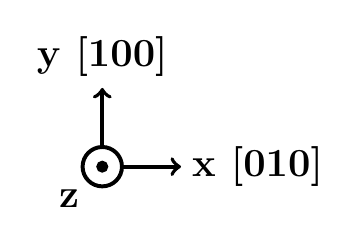
\begin{tikzpicture}
\draw [fill=white,white] (-0.8,-0.6) rectangle (2.6,1.7);
\draw[line width=0.5mm, ->] (0.25,0.00) -- (1.00,0.00)   node[anchor = west]  {\Large{\textbf{x [010]}}};
\draw[line width=0.5mm, ->] (0.00,0.25) -- (0.00,1.00)   node[anchor = south] {\Large{\textbf{y [100]}}};
\draw            (0.00,0.00)    (-0.17,-0.17) node[anchor = north east] {\Large{\textbf{z}}};
\draw[line width=0.5mm] (0,0) circle [radius=0.25];
\draw[line width=0.5mm, fill=black] (0,0) circle [radius=0.05];
\end{tikzpicture}
\end{figure}

\end{document}
0.17
